\documentclass[10pt,twocolumn,letterpaper]{article}
\usepackage{cvpr}
% The report uses only the packages loaded in main.tex and cvpr.sty.

\usepackage{graphicx,booktabs,amsmath}
\definecolor{cvprblue}{rgb}{0.21,0.49,0.74}
\usepackage[breaklinks,colorlinks,allcolors=cvprblue]{hyperref}
\graphicspath{{../evidence/}}
\title{Garden Reconstruction and White-Plush Integration}
\author{CIE6004 Assignment 2}
\begin{document}
\maketitle
\begin{abstract}
We reconstruct the Garden scene with 3D Gaussian Splatting and the supplied white plush with an object-centric MILo model~\cite{milo}, then place the resulting surface in the Garden. The Garden model improves all three public validation metrics over the supplied baseline. For the plush, a conservative cull guided only by training silhouettes raises mean held-out silhouette IoU from 0.617 to 0.936. A fixed object-to-scene transform seats the plush on the tabletop while a one-way 180-degree camera half-turn carries it behind the vase and reveals it again. Per-pixel Garden depth confirms occlusion across the full 240-frame clip. Clip 1980 and Garden test references were not opened.
\end{abstract}

\section{Data and protocol}
Garden training uses 161 supplied views; its 12 public validation references are used only for metric self-checks. We train the scene model on all 161 images and render the 12 required test camera poses without accessing test references. The object is the supplied white plush. From clips 1978 and 1979, the fixed development split contains 143 training views and 12 validation views (1979 frames 48--70 at stride 2). Validation images and masks are stored outside the MILo training image directory. The reserved clip 1980 was not opened or copied. Four user-reviewed training masks anchor paw and cloth boundaries; 39 masks are propagated from these anchors and 100 use independent SAM2 image prompts~\cite{sam2}.

\section{Garden reconstruction}
We initialize the scene from 135,521 COLMAP points and optimize the 161 training views with 3D Gaussian Splatting~\cite{kerbl} for 30,000 steps on one NVIDIA RTX A6000 (physical GPU 4). Training takes 1,998.6 s; the model grows to 4.92 million Gaussians. The mean training loss falls from 0.2945 to 0.0389. Table~\ref{tab:garden} reports public validation metrics.
\begin{table}[t]\centering\small
\caption{Mean metrics over 12 public Garden validation views.}\label{tab:garden}
\begin{tabular}{lrrr}\toprule
Model & PSNR$\uparrow$ & SSIM$\uparrow$ & LPIPS$\downarrow$ \\\midrule
Supplied baseline & 25.726 & 0.7925 & 0.17568 \\
Our Garden model & \textbf{27.029} & \textbf{0.8592} & \textbf{0.08371} \\\bottomrule
\end{tabular}\end{table}
All three metrics improve. DSC07988 is the hardest public validation view by PSNR (19.80 dB). The render preserves the foreground table, but gaps and dark artifacts appear along the upper background canopy (Fig.~\ref{fig:garden-hardest}).
\begin{figure}[t]
\centering
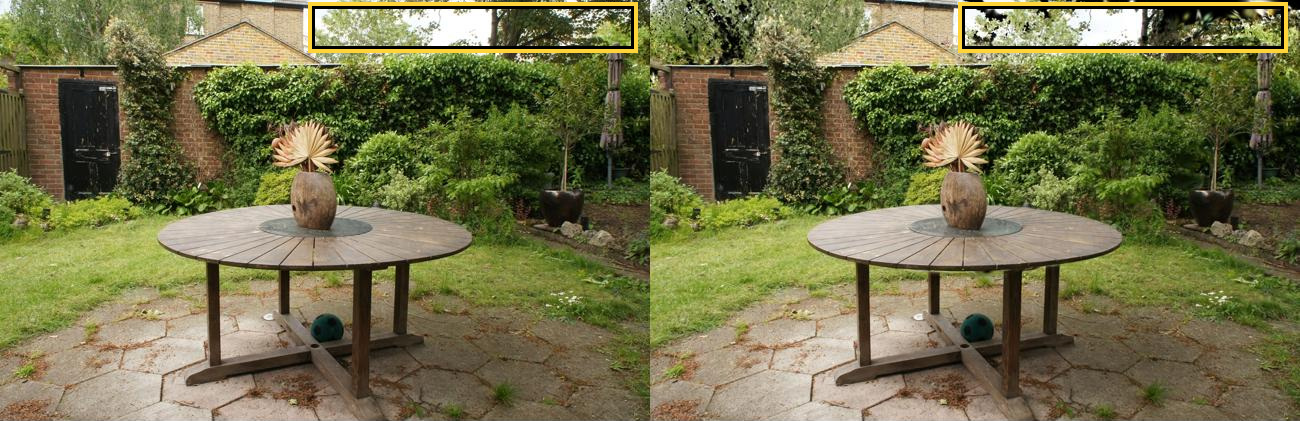
\includegraphics[width=\linewidth]{garden_validation_DSC07988.jpg}
\caption{Garden validation view DSC07988. Left: reference photograph. Right: our 3DGS render. The boxes mark the same canopy region, where the render shows dark gaps along the top edge.}
\label{fig:garden-hardest}
\end{figure}

\section{White-plush reconstruction}
We rebuild cameras from the 143 training images only (143/143 registered; 23,108 sparse points) using a train-only COLMAP map~\cite{sfm}, then register the 12 held-out views separately by PnP. MILo trains for 30,000 iterations on one RTX A6000 (GPU 4) in 49 min 18 s. Its input uses the four reviewed masks, their 39 propagated masks, and 100 SAM2 image masks. The final learned-SDF mesh is culled using training cameras and masks only. It contains 199,712 vertices and 398,449 faces, with zero non-manifold edges and 1,345 boundary edges; it is open and is not watertight.
\begin{figure}[t]\centering
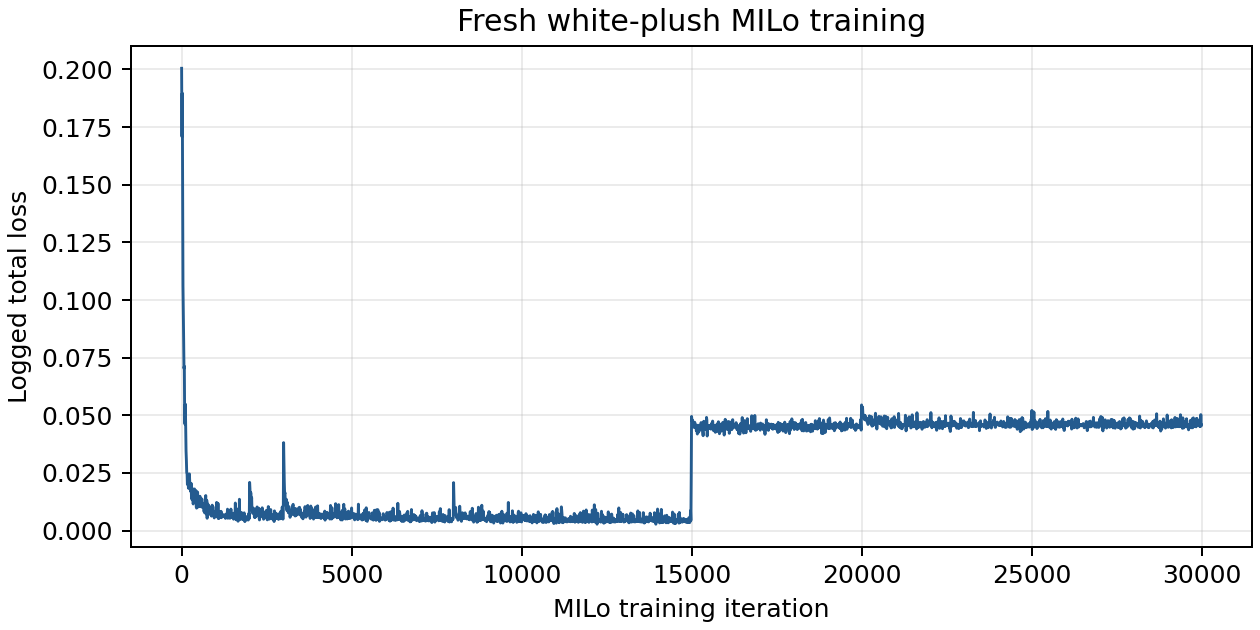
\includegraphics[width=\linewidth]{loss.png}
\caption{Logged total loss during the 30k-iteration white-plush MILo run.}\label{fig:loss}
\end{figure}

The baseline defect is silhouette leakage: the raw mesh produces thousands of rendered surface hits outside the reference mask in each validation view. We hypothesize that these overextended surface regions come from weakly constrained geometry beyond the observed silhouettes. With the split and 30k-iteration training budget fixed, we apply one change after training: conservative face culling using training cameras and masks only. On the same 12 held-out views, mean silhouette IoU rises from 0.617 to 0.936 (Fig.~\ref{fig:ablation}); per-view scores improve consistently. Matched renders at two held-out poses show the same effect (Fig.~\ref{fig:paired}): IoU rises from 0.613 to 0.948 at frame 1979\_000048 and from 0.583 to 0.941 at frame 1979\_000070. The change reduces silhouette leakage, while the remaining open boundary (1,345 edges) and coarse fur geometry show that silhouette agreement does not establish watertightness or fine surface detail.
\begin{figure*}[t]\centering
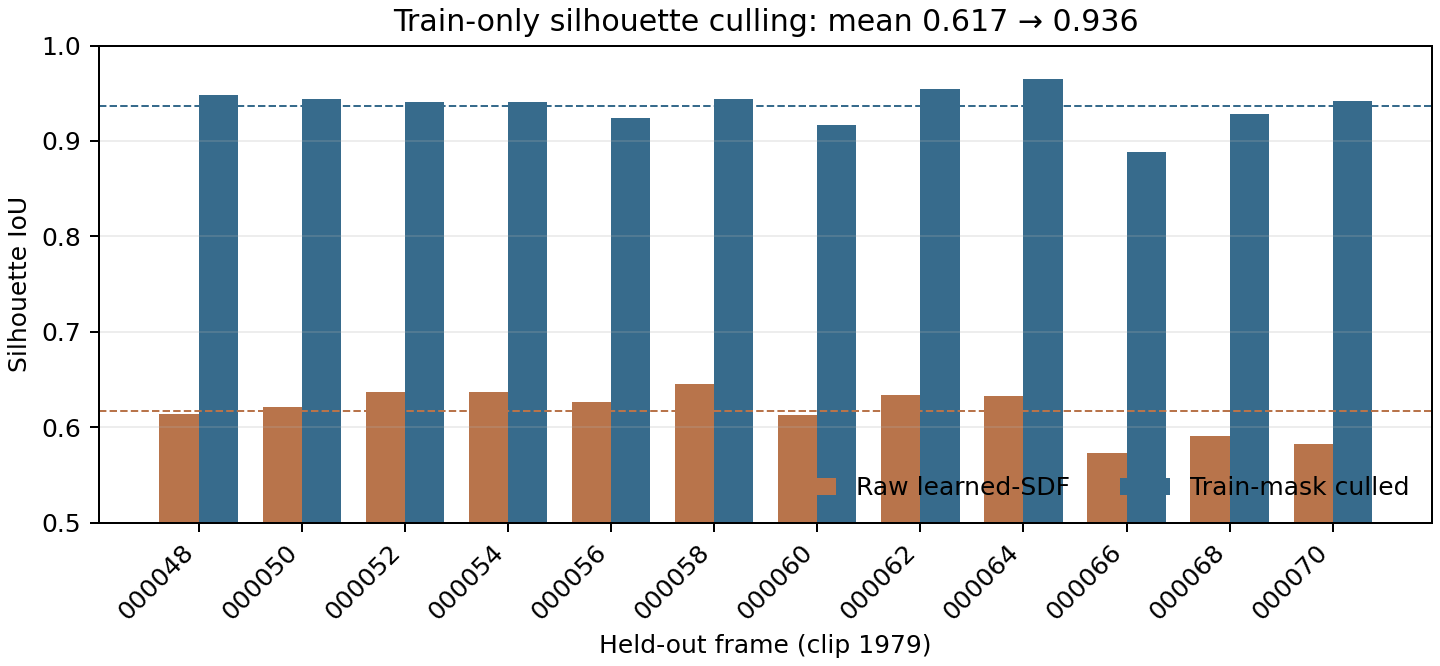
\includegraphics[width=.78\textwidth]{ablation.png}
\caption{Held-out silhouette IoU before and after the training-only cull. Geometry is evaluated with the same 12 validation views.}\label{fig:ablation}
\end{figure*}

\begin{figure*}[t]\centering
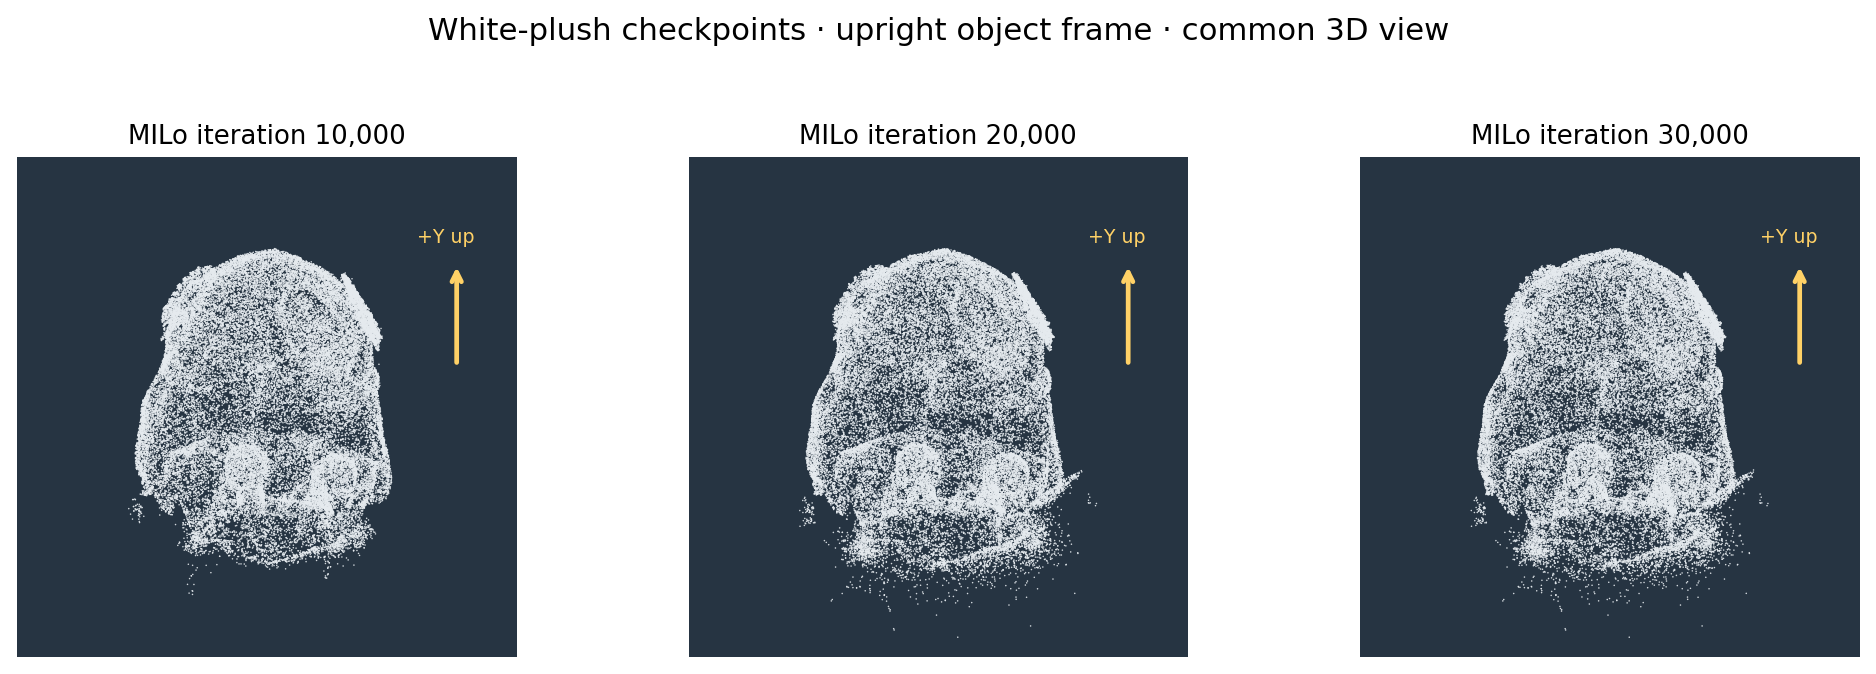
\includegraphics[width=.93\textwidth]{stages.png}
\caption{Saved MILo point-cloud checkpoints at 10k, 20k, and 30k iterations, expressed in the object frame established by the source-view orientation check. The indicated $+Y$ direction is head-up; every panel shares the same 3D camera and coordinate limits. 50k points are sampled only for display.}\label{fig:stages}
\end{figure*}
\begin{figure*}[t]\centering
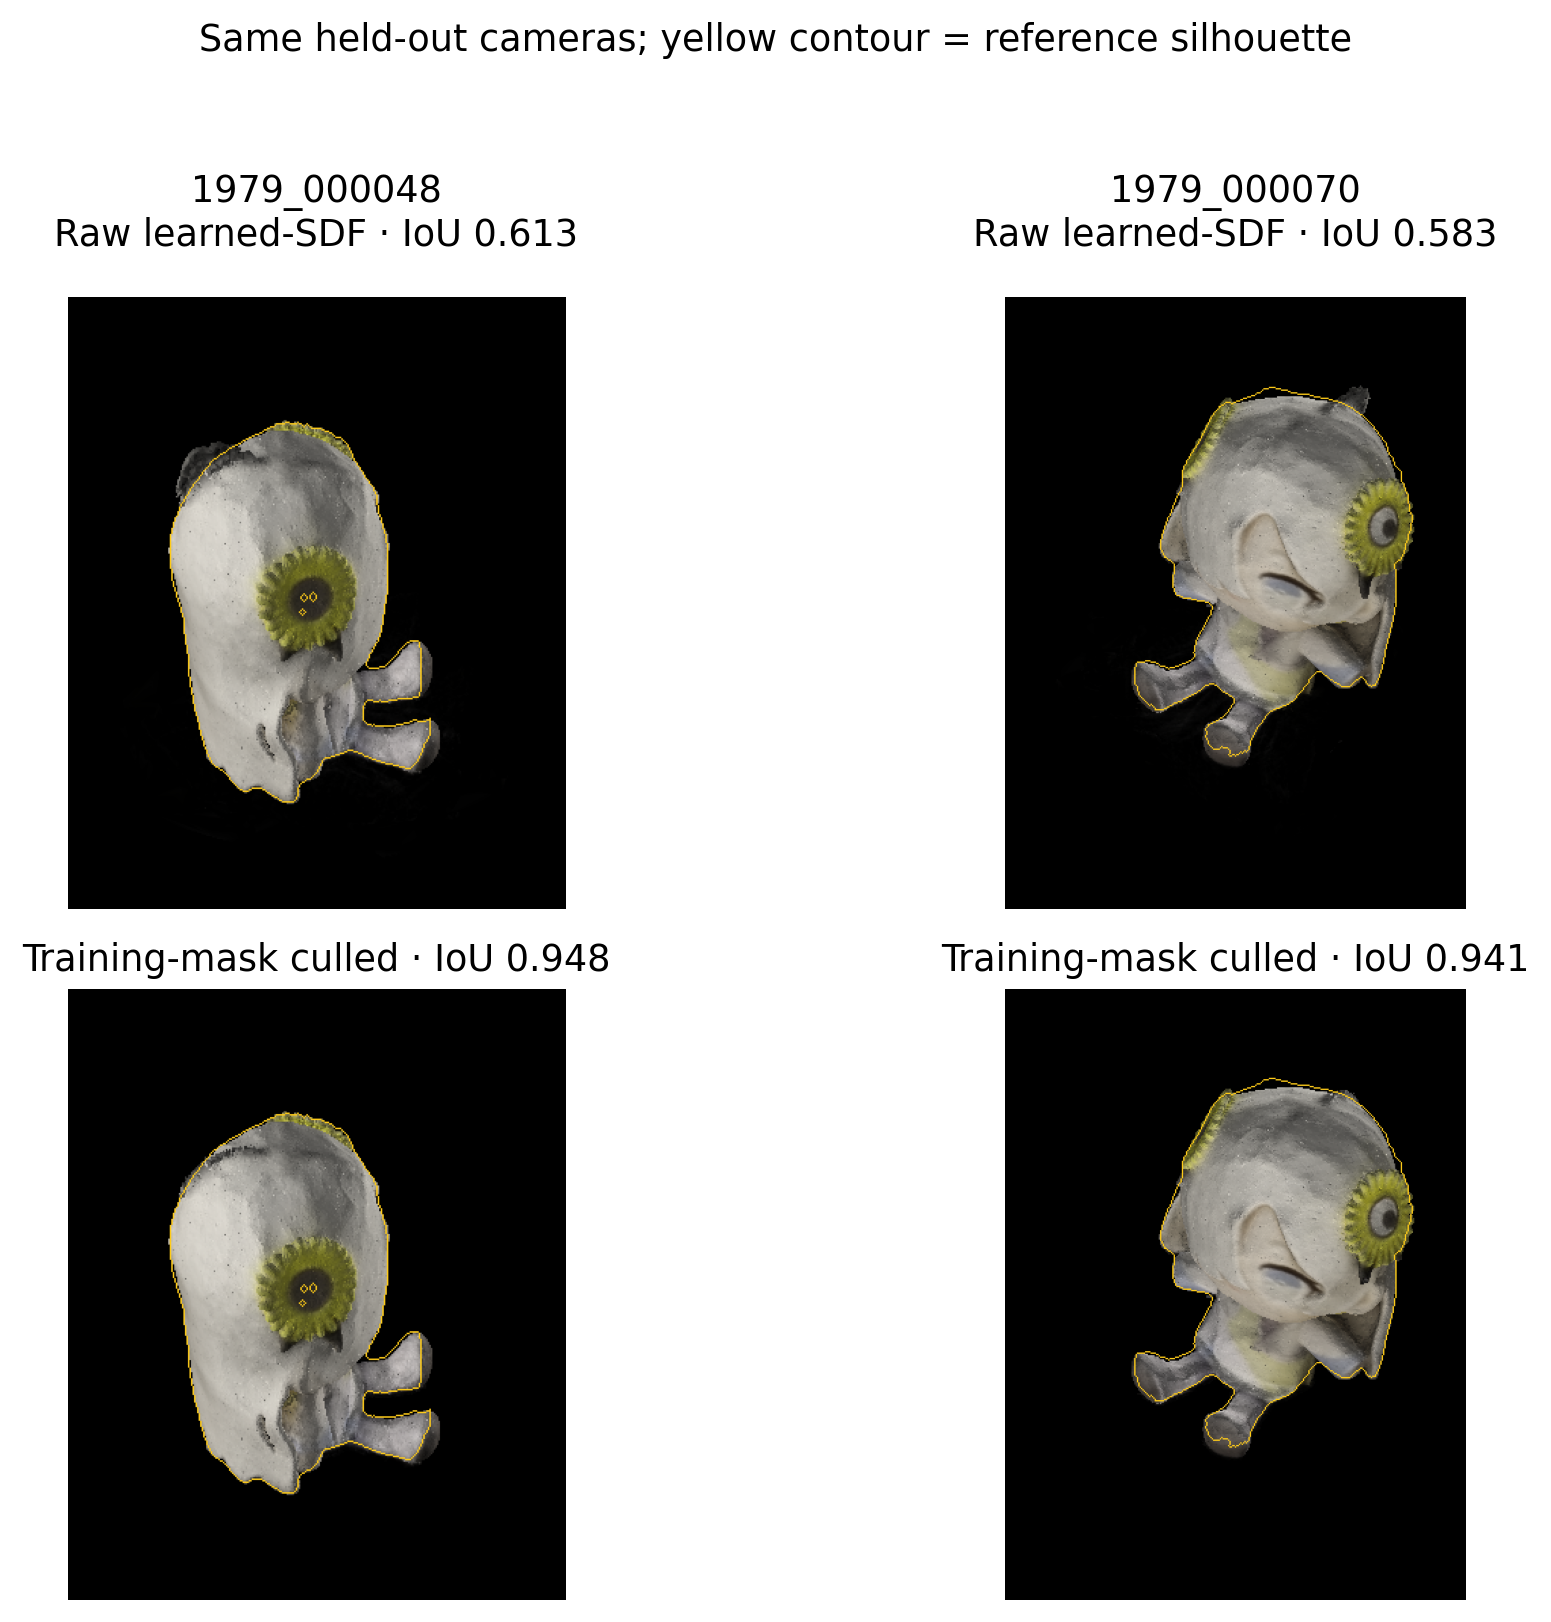
\includegraphics[width=.82\textwidth]{matched_view_comparison.png}
\caption{Baseline and train-mask-culled meshes at the same two held-out camera poses. Top: raw learned-SDF; bottom: culled mesh. The yellow contour is the reference silhouette. IoU is computed at stride 2.}
\label{fig:paired}
\end{figure*}
\section{Placement and fusion}
\begin{figure*}[t]\centering
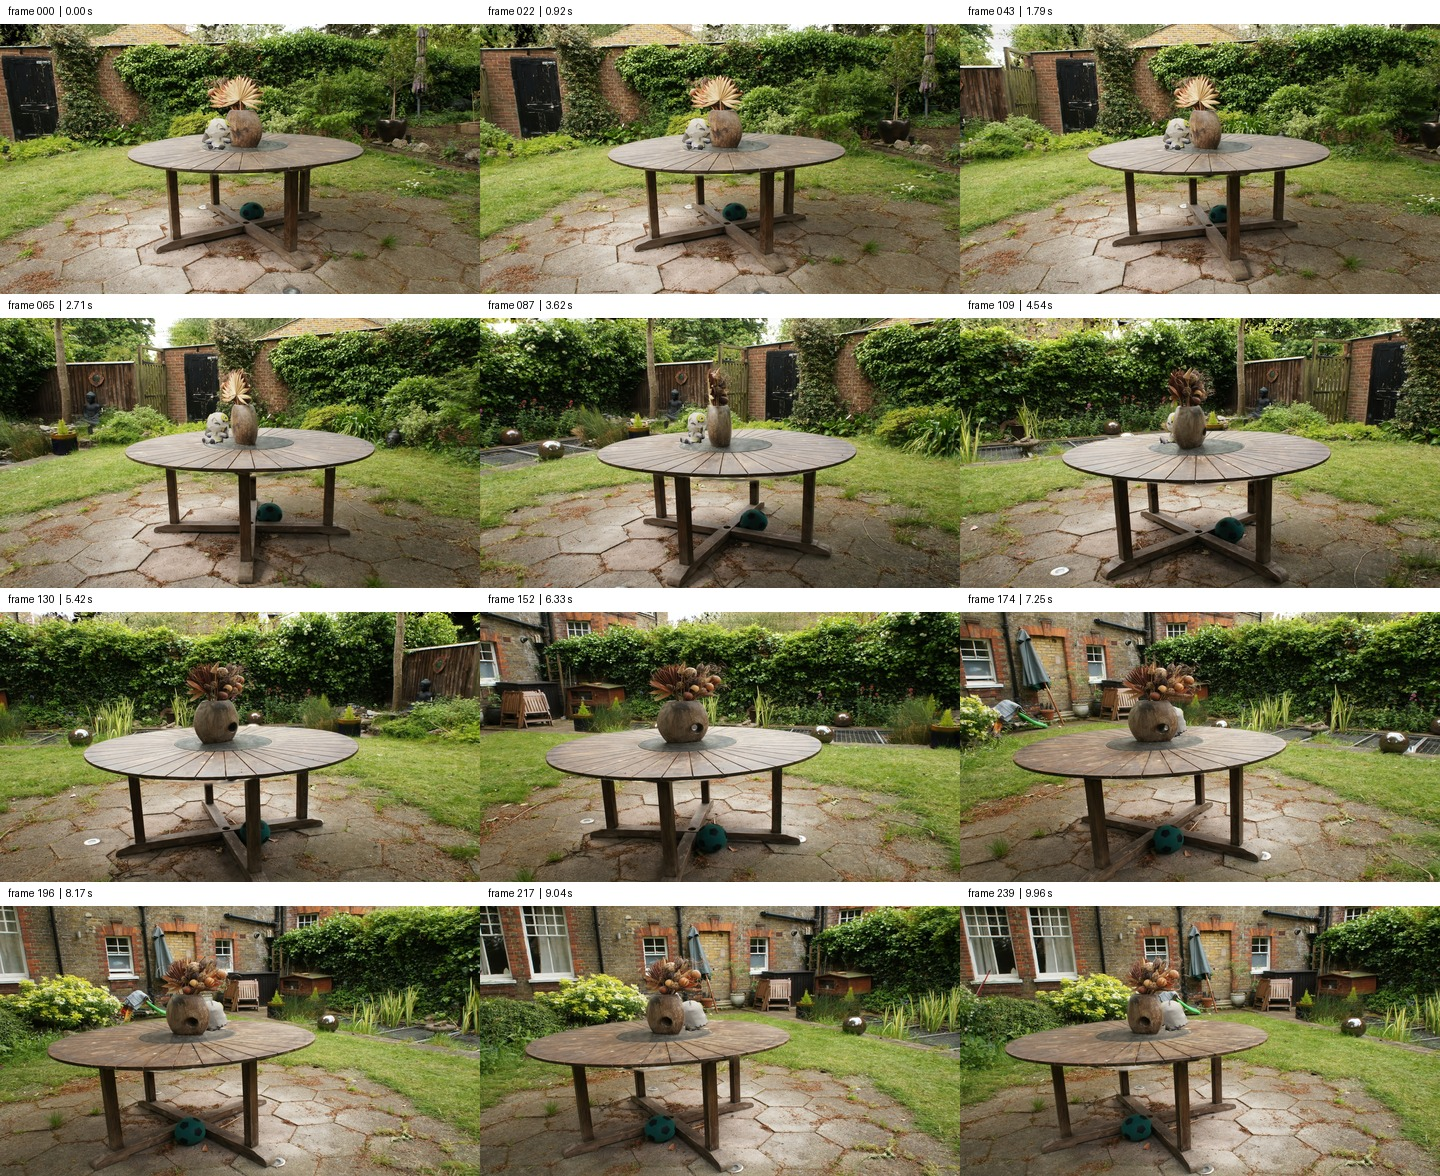
\includegraphics[width=.93\textwidth]{fusion_orbit_review.jpg}
\caption{Sampled frames from the final fixed-transform half-turn. The plush starts visible, passes behind the vase, and reappears near the end.}\label{fig:fusion}
\end{figure*}

We fit the Garden tabletop with RANSAC followed by total least squares (5,167 inliers; 0.025 scene-unit threshold). The object frame is defined with its measured support axis aligned to the fitted table normal. We scale it to 15\% of the table span (0.4138 scene-unit height), seat its support 0.005 units above the plane, and target its surface-area centroid at pixel (580, 335) in DSC07956. The support patch remains inside the table hull with a 0.562-unit margin. The same object-to-scene matrix is applied throughout the 10-second, 24-fps sequence; only the camera makes one smooth 180-degree turn. The 1296$\times$840 H.264 output contains no zoom or object-transform animation.

Figure~\ref{fig:fusion} shows sampled frames. The Garden-depth audit finds scene occlusion in 153 of 240 frames (437,941 occluded mesh pixel-frames). The plush begins fully visible, falls to 7.0\% visibility at frame 120, is fully hidden for frames 129--138, then reappears to 88.1\% visibility in the final frame. Table-depth conflicts are separately suppressed so the fitted support surface does not falsely cover the inserted mesh. The object remains upright and fixed in Garden coordinates for every frame. The composite reuses captured mesh color and the Garden's baked appearance; it does not synthesize cast shadows or relight either source.

\section{Limitations}
Garden quality is assessed on public validation views; held-out test references remain unopened. Plush validation measures silhouette agreement, and the open mesh boundary and coarse fur geometry limit confidence in unseen surface detail. Garden appearance is less reliable in reverse-side novel views. The composite uses captured mesh color and baked scene appearance, so it lacks newly synthesized contact shadows and physically consistent relighting.

\begin{thebibliography}{5}\footnotesize
\bibitem{kerbl} B. Kerbl et al. 3D Gaussian Splatting for Real-Time Radiance Field Rendering. ACM TOG, 2023.
\bibitem{sfm} J. L. Sch\"onberger and J.-M. Frahm. Structure-from-Motion Revisited. CVPR, 2016.
\bibitem{milo} A. Gu\'edon et al. MILo: Mesh-In-the-Loop Gaussian Splatting. ACM TOG, SIGGRAPH Asia, 2025.
\bibitem{sam2} N. Ravi et al. SAM 2: Segment Anything in Images and Videos. arXiv:2408.00714, 2024.
\end{thebibliography}
\end{document}


